\subsection{実験2 ジェスチャー分類問題における入力速度変化に対するモデル精度評価}
提案手法をジェスチャー動画分類問題に適用し, 未学習の入力速度に対するモデル精度評価を行う.

\subsubsection{データセット}
ジェスチャー動画のデータセットとして, SNNの評価で広く用いられる\cite{massa2020efficient}DVSGesture\cite{dvsgesture}を使用した.
DVSGestureはイベントベースビジョンセンサ (DVS128 : \figref{fig:dvs128}) で記録されている.
このセンサでは各ピクセルの輝度変化を非同期に捉え, その変化をイベント$\epsilon$として記録する (\eqrefc{eq:dvs:event}).
\begin{equation}
    \epsilon = (x, y, t, p) \label{eq:dvs:event}
\end{equation}
ここで, $(x, y)$はピクセルの座標, $t$はイベントが発生した時刻である.
また, $p$はイベント強度を表し, ピクセルの輝度変化が正であれば1, 負であれば-1の値を持つ.

イベントベースビジョンセンサによるジェスチャー記録の様子を\figref{fig:dvs:recordview}に示す.
上段が通常のフレームベースカメラで記録したもの, 下段がイベントベースビジョンセンサで記録したものである.
また, 黒色は値が0であることを表し, 青色, 桃色はそれぞれ$p=1, p=-1$のイベントを表す.
イベントは時間的なピクセルの輝度変化を検出するため, ジェスチャーでは動きの多い腕周りのピクセル情報が多く記録される.
% 画像引用元
% https://docs.inivation.com/_static/hardware_guides/dvs128.pdf
\begin{figure}[htbp]
    \centering
    \includesvg[width=0.5\textwidth, inkscapelatex=false]{Static/chap2_sec3_dvs128}
    \caption{DVS128\cite{dvs128fig}}
    \label{fig:dvs128}
\end{figure}

\begin{figure}[htbp]
    \centering
    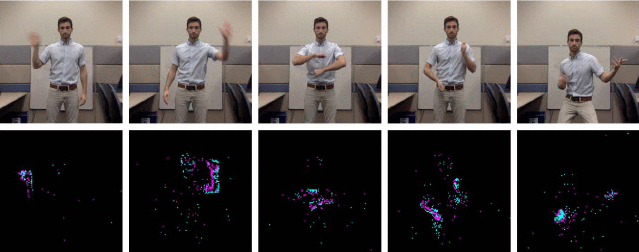
\includegraphics[width=1.0\textwidth]{Static/chap2_sec3_dvs_recordview.png}
    \caption{DVSGesture記録の様子\cite{dvsgesture}}
    \label{fig:dvs:recordview}
\end{figure}

DVSGestureは11種類のクラスのジェスチャーを記録している.
それぞれのジェスチャーのスナップショットを\figref{fig:dvs:gesture}に示す.
\begin{figure}[htbp]
    \centering
    \includesvg[width=0.5\textwidth, inkscapelatex=false]{dummy/dummy_img}
    \caption{各ジェスチャーのスナップショット}
    \label{fig:dvs:gesture}
\end{figure}


\subsubsection{モデルの学習}
モデルの学習はイベントの時系列データを入力, ジェスチャーのクラスを出力とする分類問題として行う.
ここで, 使用するデータセットのイベントの有無をスパイクとして扱うことでSNNの入力としている.
